Khi tìm hiểu về chủ thể này, sự thâm nhập của thuật toán vào lĩnh vực sinh học nói chung là cực kỳ thú vị. Trong mục này, bài viết xem thuật toán dưới góc nhìn di truyền nên những kiến thức có liên quan đến di truyền cũng sẽ được đề cập.

\subsubsection{Di truyền, ADN và nhiễm sắc thể}
Di truyền là hiện tượng truyền đạt các tính trạng của các (bố mẹ, tổ tiên) cho các thế hệ con cháu theo \cite{whatIsGenetic}.

ADN là phân tử mang thông tin di truyền quy định mọi hoạt động sống theo \cite{whatIsDNA}

Nhiễm sắc thể là bào quan chính chứa bộ gen của sinh vật, là cấu trúc quy định sự hình thành protein, có vai trò quyết định trong di truyền theo \cite{whatIsChronosome}. Có thể hiểu nhiễm sắc thể (NST) là một tập hợp của các gen.

Như vậy, mối quan hệ giữa các khái niệm có thể được mô tả theo sơ đồ sau:
\begin{figure}[h]
	\centering
	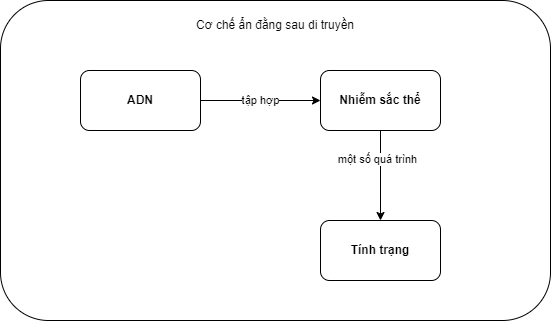
\includegraphics[scale=0.5, height=8cm]{figures/genetic_illustration_diagram.png}
	\caption{Sơ đồ mối quan hệ giữa các khái niệm. Về cơ bản ADN/NST qua một số giai đoạn trung gian để có thể biểu thị nên tính trạng. Và quá trình đó có thể hiểu là cơ chế biểu thị của di truyền}
	\label{fig:genetic_illustration_diagram}
\end{figure}

\noindent
Việc đề cập đến kiến thức di truyền nhằm khẳng định vai trò của di truyền là mang \textbf{tính hướng dẫn}. Điều này tương tự với nội dung đã đề cập trong định nghĩa của thuật toán \ref{sec:algorithm}.

Về bản chất của áp dụng trong mục này là nhận ra ADN/NST là có tính hướng dẫn tương tự như thuật toán. Sự suy luận này xuất phát từ việc đúc kết những đối tượng mang tính tương tự thường sẽ có một số tính chất chung.

Vậy câu hỏi mà mục này đặt ra là: "\textbf{Mình khai thác tính hướng dẫn mà sinh học nói chung mang lại cho thuật toán như thế nào?}"

